%% ------------------------------------------------------------------------- %%
\chapter{Resultados}
\label{cap:resultados}

Neste capítulo apresentamos os resultados da avaliação do uso das redes convolucionais na recuperação de trecho de código-fonte. Utilizamos a nossa arquitetura proposta no Capítulo~\ref{cap:abordagem} e comparamos com outras duas arquiteturas: uma arquitetura de referência \textit{Embedding} e outra arquitetura que é o estado da arte em recuperação de trecho de código proposta por \cite{cambronero-deep-learning-code-search:2019}. Os resultados da arquitetura CNN foram promissores. A arquitetura apresentou um valor de métrica \acrfull{mrr} de $0,70$. Em $78\%$ das vezes, as respostas corretas apareceram entre as 3 primeiras posições, de um total de 50 possíveis respostas.

\section{Avaliação}
\label{sec:resultados-avaliacao}

Avaliamos a arquitetura CNN juntamente com outras duas arquiteturas, Embedding e \Gls{unif} na recuperação de trecho de código-fonte através do procedimento proposto por \cite{iyer-etal-2016-summarizing} e descrito na Seção~\ref{sec:avaliacao}. Os resultados foram coletados a partir da amostra \emph{EVAL} e o valor final MRR é a média obtida após 20 iterações. Conforme a Tabela~\ref{table:resultados}, as arquiteturas CNNs compartilhadas com 4000 filtros convolucionais (linhas D3 e G3) obtiveram o melhor resultado. A arquitetura CNN obteve uma média MRR 5\% superior ao melhor resultado obtido pela arquitetura Unif (linha B1), atual estado da arte, e um resultado 11\% superior a arquitetura de referência Embedding (linha A1). 

\begin{table}[H]
\centering
\begin{tabular}{ p{1cm} p{6cm} P{4cm} P{4cm} }
 \hline
    & & \multicolumn{2}{c}{\textbf{Resultados}}\\
 \hline
 & \textbf{Modelos} & \textbf{MRR} & \textbf{TOP1}\\
 \hline
 A1 & Embedding (m = $0.1$) & $0.637$& $0.493 \pm 0.009$\\
 
 \hline
 
 B1 & Unif (m = $0.2$) & $0.675 \pm 0.006$ & $0.539 \pm 0.009$\\
 
 \hline
 
 C1 & CNN / F = 1000 & $0.669 \pm 0.006$ & $0.527 \pm 0.012$\\
 
 C2 & CNN / F = 2000 & $0.673 \pm 0.007$ & $0.531 \pm 0.012$\\
 
 C3 & CNN / F = 4000 & $0.687 \pm 0.006$ & $0.553 \pm 0.011$\\
 
 \hline
 
 D1 & CNN Compartilhado / F = 1000 & $0.678 \pm 0.007$ & $0.548 \pm 0.012$\\
 
 D2 & CNN Compartilhado / F = 2000 & $0.694 \pm 0.008$ & $0.565 \pm 0.012$\\
 
 D3 & CNN Compartilhado / F = 4000 & $0.700 \pm 0.004$ & $0.569 \pm 0.009$\\
 
 
 
 \hline
 
 E1 & Unif (m = $0.05$) com NL & $0.653 \pm 0.006$ & $0.515 \pm 0.011$\\
 
 \hline
 
 F1 & CNN com NL / F = 1000 & $0.682 \pm 0.007$ & $0.543 \pm 0.012$\\
 
 F2 & CNN com NL / F = 2000 & $0.689 \pm 0.006$ & $0.553 \pm 0.011$\\
 
 F3 & CNN com NL / F = 4000 & $0.688 \pm 0.006$ & $0.553 \pm 0.011$\\
 
 \hline
 
 G1 & CNN Compartilhado com NL / F = 1000 & $0.690 \pm 0.008$ & $0.553 \pm 0.015$\\
 
 G2 & CNN Compartilhado com NL / F = 2000 & $0.700 \pm 0.007$ & $0.573 \pm 0.012$\\
 
 G3 & CNN Compartilhado com NL / F = 4000 & $0.701 \pm 0.008$ & $0.577 \pm 0.015$\\
 
\hline
\end{tabular}
\caption{Resultado do modelo CNN em comparação com as outras arquiteturas \Gls{unif} e Embedding. MRR refere-se a média do resultado do Mean Reciprocal Rank (equação~\ref{eq:mrr}) na amostra EVAL. TOP1 refere-se a frequência da ocorrência da resposta anotada como correta na primeira posição em comparação com outros 49 distratores. Nas linhas A1, B1 e E1, \emph{m} refere-se ao hiper-parâmetro margem utilizada na função de perda \emph{hinge}. F indica a quantidade de filtros convolucionais utilizados durante o treinamento das redes convolucionais. NL é o acrônimo de normalização em lote. As arquiteturas CNN utilizaram margem $m = 0.05$ e o tamanho da janela do filtro (kernel) $k = 2$.}
\label{table:resultados}
\end{table}

Conforme os resultados da Tabela~\ref{table:resultados}, os ajustes dos hiper-parâmetros para a arquitetura CNN foram ao encontro de \cite{tan-lstm-qa, feng-2015}, no qual verificaram que o aumento da quantidade de filtros convolucionais, que aumenta a capacidade das redes convolucionais e as características latentes a serem extraídas, resultaram em uma melhora no desempenho do modelo (linhas D3 e G3). Além disso, verificamos que o valor $2$ para o tamanho da janela dos filtros obteve os melhores resultados, não havendo melhora significativa para janelas de tamanho $3$ ou $4$. E diferentemente do apontamento feito por \cite{tang-hybrid-deep-representation-2018}, não notamos melhora no desempenho através da combinação de filtros com janelas de tamanhos diferentes, e.g., $2,3,5,7$ (ver Apêndice~\ref{ape:ajuste-hiper-parametros-cnn}). Porém com relação a margem utilizada na função de perda hinge, as redes convolucionais obtiveram um resultado melhor com $0.05$, já Unif obteve o melhor resultado com $0.2$ e enquanto Embedding obteve com $0.1$ (ver Apêndice~\ref{ape:ajuste-hiper-parametros-cnn}). No caso de \cite{tan-lstm-qa} ele fixou a margem em $0.2$.


Conforme verificado por \cite{tan-lstm-qa} e \cite{feng-2015}, as redes convolucionais que compartilham os parâmetros dos pares de questões e respostas durante a aprendizagem (linhas D e G) obtiveram um desempenho superior aos modelos que utilizaram parâmetros independentes (linhas C e F). Conforme \cite{tan-lstm-qa}, os parâmetros indepdendentes tornam a aprendizagem mais difícil, pois o otimizador terá que aprender o dobro de parâmetros. Já para \cite{wen-joint-modeling-question-answer-2019}, as redes convolucionais que aprendem as representações de forma independente e postergam a interação entre elas para a última camada (cálculo da similaridade e função de perda \textit{hinge}), exploram de forma ineficiente a correlação semântica entre as respectivas representações dos pares de questões e respostas. No nosso caso, verificamos que ao treinar por mais épocas, não houve melhora significativa no desempenho, salientando a dificuldade das redes convolucionais que aprendem as representações de forma independente em encontrar uma correlação semântica entre os pares de questões e respostas.

Durante o treinamento, para evitar o \textit{overfitting} dos modelos, adotamos a técnica de normalização em lote, que além de melhorar o desempenho, a velocidade e a estabilidade das redes neurais, ele mitiga o \textit{overfitting}, reduzindo a necessidade do uso de outra técnica de regularização como o \textit{dropout} \citep{sergey-batch-normalization-2015}. No nosso caso, verificamos a melhora no desempenho e robustez do modelo nas redes convolucionais (ver linhas F e G da Tabela~\ref{table:resultados} e ver Apêndice~\ref{ape:ajuste-hiper-parametros-cnn}). No caso da arquitetura Unif proposta por \cite{cambronero-deep-learning-code-search:2019}, não notamos melhora significativa no desempenho, somente na robustez do modelo.


Para entender um pouco melhor o resultado da média harmônica MRR, a Figura~\ref{fig:histogram-mrr} exibe as posições da primeira ocorrência do trecho de código-fonte encontradas durante a avaliação dos modelos.

\begin{figure}[h]
    \centering
    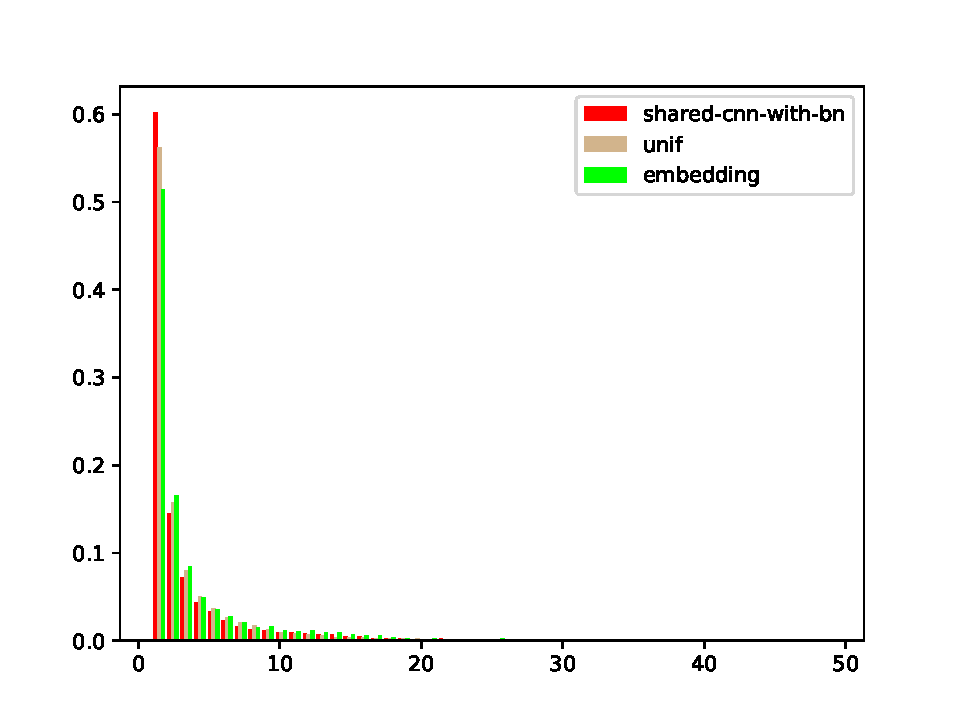
\includegraphics[width=1\textwidth]{figuras/cap-resultados/histogram.pdf}
    \caption{Figura das primeiras posições observadas para o trecho de código-fonte anotado como correto. As legendas \emph{shared-cnn-with-bn}, \emph{unif} e \emph{embedding} referem-se as linhas G3, A1 e B1 da Tabela~\ref{table:resultados} respectivamente.}
    \label{fig:histogram-mrr}
\end{figure}


Tanto o CNN quanto a arquitetura Unif conseguiram classificar os trechos de código-fonte entre as 3 (três) primeiras posições em 75\% dos casos. A nossa arquitetura proposta obteve uma precisão TOP-1 de aproximadamente 60\%, i.e., em aproximadamente 60\% das vezes, o trecho de código-fonte relevante ficou na primeira posição. Já a arquitetura Unif e Embedding obtiveram uma precisão TOP-1 de pouco mais de 50\%. Um ponto a ser levantado é que a nossa métrica MRR só leva em consideração a posição apontada pelo modelo para o trecho de código-fonte anotado como correto. Mesmo que o modelo apresente um outro trecho de código-fonte que também é solução, o nosso método de avaliação não leva em consideração. Neste caso, o modelo é penalizado.



\section{Ameaças à validade}

Conforme citado anteriormente, \cite{yao-2018} anotaram o conjunto de dados utilizando um framework proposto em seu artigo. Para anotá-los, os autores treinaram uma rede neural no conjunto de dados anotado manualmente. Em nosso trabalho, fizemos o caminho inverso. Treinamos os nossos modelos nos dados anotados automaticamente e avaliamos no conjunto anotado manualmente. Para diminuir o viés, adotamos o procedimento proposto por \cite{iyer-etal-2016-summarizing} descrito na Seções~\ref{sec:treinamento} e \ref{sec:avaliacao}.

\section{Considerações}

Os resultados foram muito promissores, as arquiteturas propostas obtiveram um bom desempenho na recuperação de trecho de código-fonte. Algumas considerações a respeito do experimento e dos resultados das redes convolucionais:

\begin{itemize}
    \item Não houve a necessidade de um tratamento especial para os trechos de código em Python, devido as suas características como sintaxe mais concisa, clara e muito menos verbosa quando comparada a outras linguagens \citep{theodora-introductory-programming-python-2015}, facilitando a extração das palavras durante o pré-processamento. 
    
    \item Isto nos ajudou também a implementar de forma mais rápida as abordagens já conhecidas em \acrshort{nlp} \citep{feng-2015, tan-lstm-qa}. E mostrou um possível caminho para a criação de uma busca semântica de trecho de código utilizando aprendizagem de representação. No nosso caso, utilizamos \Gls{word2vec}, mas recentes avanços em NLP apresentaram outras soluções como \acrshort{elmo}, \acrshort{bert} e o mais recente \Gls{xlnet} \citep{yang2019xlNet, devlin-etal-2019-bert}. Trabalhos futuros podem investigar como estes recentes avanços podem auxiliar na recuperação de trecho de código-fonte.
    \item Conforme apontado por \cite{tom-young:trends-deep-learning-nlp}, as redes convolucionais tentam extrair os n-grams mais importantes e dão prioridade às interações locais. E apesar de \cite{tom-young:trends-deep-learning-nlp} ter observado em outros trabalhos que o CNN tem dificuldades em inferir o contexto em sentenças curtas, no nosso caso, o uso de vetores de representação distribuída ajudou a rede convolucional a extrair a semântica do trecho de código correlacionando-a à questão. Adotamos o mesmo procedimento de \cite{tan-lstm-qa} e criamos uma matriz de representação distribuída comum a partir da junção do vocabulário das questões e dos trechos de código, ver Seção~\ref{sec:abordagem-representacao-token}.
    \item Segundo \cite{Goodfellow-et-al-2016:convolutional-networks}, as redes convolucionais não conseguem correlacionar palavras muito distantes em um sentença. No nosso caso, isto não foi um problema, pois conforme apontado na Tabela~\ref{table:statistical-descriptive-of-pythons-sample}, 75\% das questões das nossas amostras tem 11 palavras no máximo, enquanto 75\% dos trechos de código tem no máximo 55 palavras, i.e., tanto as questões e as respostas são relativamente curtas. Por exemplo, o conjunto de dados \acrshort{squad}, que contém mais de $100.000$ questões e respostas coletadas de artigos do Wikipedia, apresenta em média 15 palavras para as questões e 150 para as respostas, i.e., praticamente o dobro do tamanho das questões que utilizamos e o triplo de palavras do trecho de código-fonte \citep{rajpurkar-etal-2016-squad}. 
    \item Adotamos a métrica MRR que indica o quanto um modelo está conseguindo classificar a informação relevante entre as primeiras posições. No nosso caso, a informação relevante é o trecho de código anotado como correto. Conforme o resultado apresentado na Seção~\ref{sec:resultados-avaliacao}, o valor alto do MRR indica que o modelo está conseguindo classificar o trecho anotado como correto entre as primeiras posições. No caso do CNN (linha G3 da Tabela~\ref{table:resultados}), ele conseguiu classificar o trecho anotado como correto entre as 3 primeiras posições, de um total de 50, em 78\% dos casos. Para nós, isto é um indicativo de que o modelo está atentendendo a intenção do usuário, pois a informação relevante está aparecendo entre as primeiras posições. Porém, somente a métrica MRR não é suficiente, é necessário investigar e analisar estes resultados com usuários finais. Um estudo mais minucioso e qualitativo é necessário para validar estes resultados.
\end{itemize}


